\documentclass[11pt, spanish, a4paper, twoside]{article}

% Versión 1.er cuat 2021 Víctor Bettachini < vbettachini@unlam.edu.ar >

\usepackage[T1]{fontenc}
\usepackage[utf8]{inputenc}

% \usepackage[spanish, es-tabla]{babel}
\def\spanishoptions{argentina} % Was macht dass?
% \usepackage{babelbib}
% \selectbiblanguage{spanish}
% \addto\shorthandsspanish{\spanishdeactivate{~<>}}

\usepackage{graphicx}
\graphicspath{{./figuras/}{../LaTeX/}{../figurasLaTeX/}}
% \usepackage{float}

\usepackage[arrowdel]{physics}
\newcommand{\pvec}[1]{\vec{#1}\mkern2mu\vphantom{#1}}
% \usepackage{units}
\usepackage[separate-uncertainty= true, multi-part-units= single, range-units= single, range-phrase= {~a~}, locale= FR]{siunitx}
\usepackage{isotope} % $\isotope[A][Z]{X}\to\isotope[A-4][Z-2]{Y}+\isotope[4][2]{\alpha}

\usepackage{tasks}
\usepackage[inline]{enumitem}
% \usepackage{enumerate}

\usepackage{hyperref}

% \usepackage{amsmath}
% \usepackage{amstext}
% \usepackage{amssymb}

\usepackage{tikz}
\usepackage{tikz-3dplot}
\usepackage{tikz-dimline}
\usetikzlibrary{calc}
% \usetikzlibrary{math}
\usetikzlibrary{arrows.meta}
\usetikzlibrary{snakes}
\usetikzlibrary{decorations}
\usetikzlibrary{decorations.pathmorphing}
\usetikzlibrary{patterns}

\usepackage[hmargin=1cm,vmargin=3cm, top= 0.75cm,nohead]{geometry}

\usepackage{lastpage}
\usepackage{fancyhdr}
\pagestyle{fancyplain}
\fancyhf{}
\setlength\headheight{28.7pt} 
\fancyhead[LE, LO]{\textbf{Computational Analytical Mechanics} }
% \fancyhead[LE, LO]{\textbf{Mecánica General} }
\fancyhead[RE, RO]{\href{https://ingenieria.unlam.edu.ar/}{$\vcenter{\hbox{
\includegraphics[height=1cm]{../../../../figurasLaTeX/ambos.pdf}}}$}}  %edg fix path
\fancyfoot{\href{https://creativecommons.org/licenses/by-nc-sa/4.0/deed.es_ES}{$\vcenter{\hbox{
\includegraphics[height=0.4cm]{../../../../figurasLaTeX/by-nc-sa_80x15.pdf}}}$} \href{https://ingenieria.unlam.edu.ar/}{DIIT - UNLaM}}  %edg fix path
\fancyfoot[C]{ {\tiny Updated on \today} }
\fancyfoot[RO, LE]{Pág. \thepage/\pageref{LastPage}}
\renewcommand{\headrulewidth}{0pt}
\renewcommand{\footrulewidth}{0pt}


\begin{document}
\begin{center}
  % \textsc{\large Mecánica general}\\
  \textsc{\large Fuerzas de ligadura | Multiplicadores de Lagrange} 
\end{center}

\begin{enumerate}

	\item
	\begin{minipage}[t][1.1cm]{0.75\textwidth}
		\textbf{Péndulo rígido ideal}\\
		Calcule la tensión de la cuerda con el método de multiplicadores de Lagrange.
		La restricción es que la pesa se mantiene siempre en \(\vec{r} = \ell \hat{\rho}\), ergo la función que expresa esto es \(f(\rho) = \rho - \ell = 0\).
	\end{minipage}
	\begin{minipage}[c][0cm][t]{0.25\textwidth}
		\begin{tikzpicture}[scale= 1.0]
  		\draw [arrows=-latex] (-1,2) -> (-1,1) node [above=15, right=2] {\(\vec{g}\)}; % g vertical
			\draw [ultra thick] (-1.5,3) -- (2,3);
			\fill [pattern = north east lines] (-1.5,3) rectangle (2,3.2); % techo
			\draw [dashed] (0,3) -- (0,-.25);	% vertical
			\draw [thick] (0,3) -- +(-60:3) node[midway,above,right=2] {\(\ell\)};	% inclinada +:relativa, -60 grados, longitud 3
			\shade [ball color=black!80] ($(0,3)+(-60:3)$) circle(0.25) node [] {\color{white} $m$};
    	\draw [arrows=-latex] (0,.4) -> (1.25,.4) node [midway, above] {\( \psi \)}; % desplazamiento horizontal
			\draw [arrows=-latex] (0,0) arc [start angle=-90, end angle=-65, radius=3] node [below=12, left=8] {\( \varphi \)};
		\end{tikzpicture}
	\end{minipage}



	\item 
	\begin{minipage}[t][4cm]{0.47\textwidth}
	\textbf{Cilindro que rueda por un plano inclinado} [Marion (e) ex. 7.5]\\
	% English \textbf{Marion ejemplo 6.5 y ejemplo 7.9} Disco rodando en un plano inclinado.
		\begin{enumerate}
			\item Encuentre las ecuaciones de movimiento, 
			\item la aceleración angular,
			\item y la fuerzas de ligadura. 
		\end{enumerate}
	\end{minipage}
	\begin{minipage}[c][2.5cm][t]{0.3\textwidth}
		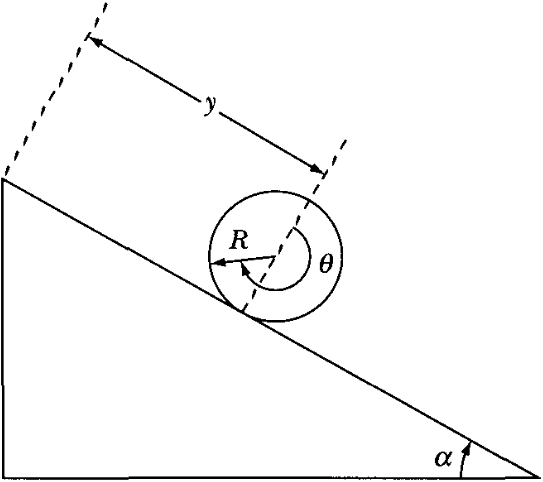
\includegraphics[width=\textwidth]{marion_fig6_7}
	\end{minipage}

	
	\item
	\begin{minipage}[t][6.5cm]{0.65\textwidth}
	\textbf{Doble máquina de Atwood} [Marion (e) ej. 7.8 y 7-37]\\
	Utilice el sistema de coordenadas indicadas.
	Para este sistema de poleas determine: 
	\begin{enumerate}
		\item las ecuaciones de movimiento,
		\item y las tensiones de ambas cuerdas utilizando el método de multiplicadores de Lagrange.
	\end{enumerate}
	Resultados:\\
	\(
		Q_{1} = \frac{g \left(32 m_{1} m_{2} m_{3} + 8 m_{1} m_{2} m_{p} + 20 m_{1} m_{3} m_{p} + 4 m_{1} m_{p}^{2} + 8 m_{2} m_{3} m_{p} + 2 m_{2} m_{p}^{2} + 4 m_{3} m_{p}^{2} + m_{p}^{3}\right)}{4 m_{1} m_{2} + 4 m_{1} m_{3} + 2 m_{1} m_{p} + 16 m_{2} m_{3} + 6 m_{2} m_{p} + 14 m_{3} m_{p} + 3 m_{p}^{2}}
	\)\\
	\(
		Q_{2} = \frac{g m_{3} \cdot \left(16 m_{1} m_{2} + 6 m_{1} m_{p} + 4 m_{2} m_{p} - m_{p}^{2}\right)}{4 m_{1} m_{2} + 4 m_{1} m_{3} + 2 m_{1} m_{p} + 16 m_{2} m_{3} + 6 m_{2} m_{p} + 14 m_{3} m_{p} + 3 m_{p}^{2}}
	\)
	\end{minipage}
	\begin{minipage}[c][0.5cm][t]{0.3\textwidth}
		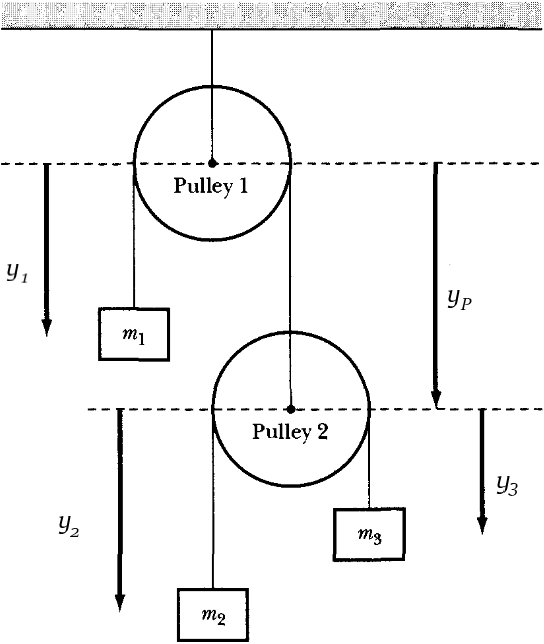
\includegraphics[width=\textwidth]{marion_fig7_6}
	\end{minipage}


	\item
	\begin{minipage}[t][6cm]{0.65\textwidth}
		\textbf{Pesos enlazados por una cuerda} [Taylor 7.50]\\
		Una partícula de de masa \(m\) posada sobre una mesa horizontal está atada a otra de masa \(M\) con una cuerda de longitud \(l\) que atraviesa un hueco en una mesa que no ofrece fricción.
		La última pende vertical con una distancia a la mesa \(y = \ell - \rho\) función de la distancia de la primera al hueco \(\rho\).
		\begin{enumerate}
			\item Asumiendo que \(\theta\) no es necesariamente constante obtenga las ecuaciones de Lagrange para \(\rho\) e  \(y\). Resultado:\\ \(- M g + M \ddot{y} + \lambda_{1} = 0 \qquad \lambda_{1} - m \rho \dot{\theta}^{2} + m \ddot{\rho} = 0\)
			\item Resuélva el sistema para \(\rho, y\) y el multiplicador de Lagrange \(\lambda_1\) encontrando las fuerzas de tensión sobre ambas masas.\\
			Resultado: \(Q_{\rho} = \frac{M m \left(g + \rho \dot{\theta}^{2}\right)}{M + m}\)
		\end{enumerate}
	\end{minipage}
	\begin{minipage}[c][0cm][t]{0.3\textwidth}
		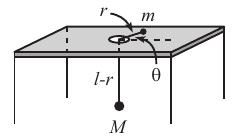
\includegraphics[width=\textwidth]{cmchap6_fig6_5}
	\end{minipage}


	\item
	\begin{minipage}[t][4.5cm]{0.62\textwidth}
		\textbf{Partícula deslizando sobre una semi-esfera} [Marion (e) ex. 7.10]\\
		La partícula de masa \(m\), considerada puntual, desliza sobre una semi-esfera de radio \(R\) sin fricción.
		\begin{enumerate}
			\item Encuentre la fuerza de la ligadura.\\
			Resultado: \(F^\mathrm{ligadura}_{\rho} = m \left(- R \dot{\theta}^{2} + g \cos{\left(\theta \right)}\right)\)
			\item Calcule el ángulo en que la partícula se despega de la semi-esfera.\\
			Resultado: \(\approx 48.19^\circ\) 
		\end{enumerate}
	\end{minipage}
	\begin{minipage}[c][0cm][t]{0.3\textwidth}
		% \includegraphics[width=\textwidth]{marion7_10}
		\begin{tikzpicture}[scale= 1.0]
			\draw [ultra thick] (-3,0) -- (3,0);
			% \draw [ultra thick] (-3,0) -- (3,0);
			\fill [pattern = north east lines] (-3,0) rectangle (3,-0.2); % piso
			\draw [ultra thick] (-2,0) .. controls (-2,2*0.555) and (-2*0.555,2) .. (0,2) .. controls (2*0.555,2) and (2,2*0.555) .. (2,0); % semi esfera
			% \filldraw (0,2.2) circle (0.2); % masa superior
			% \fill (2*0.5+.12,1.732+.18) circle [radius=0.25] node [midway, text=white] { \( m \) };
			% \filldraw (2*0.5+.12,1.732+.18) circle (0.2) node [above, right=5] {\(m\)}; % masa a la derecha
			\shade [ball color=black!80] (2*0.5+.12,1.732+.18) circle(0.2) node [] {\color{white} $m$};
			% \draw (2,2) circle [radius=0.3, color=white, fill=black] node {$T_1$};
			\draw [dashed] (0,0) -- (0,2); % linea vertical
			\draw [-LaTeX] (0,0) -- (1,1.732) node [midway, anchor=west] {\(R\)}; % linea hacia la derecha
			\draw [-stealth] (0,1) arc (90:60:1) node [above left] {\(\theta\)}; % arco c/ flecha comenzando en (0,1), de 90 a 60 grados, 1...
			% \node [circle,draw,label=60:$60^\circ$,label=below:$-90^\circ$] {\(m\)}; 
			% \node at (-2*0.5+.15,1.732+.15) [circle,draw,fill=black] {\(m\)}; 
			\draw [-stealth, thick] (-2.5,2) -> (-2.5,1) node [above=15, right=2] {\(\vec{g}\)}; % g vertical
		\end{tikzpicture}
	\end{minipage}
	
	Para llegar al ángulo de despegue debe resolver la ecuación diferencial a la que arribará tras resolver la problemática de las fuerzas de ligadura, que será $\ddot{\theta} = \frac{g \sin(\theta)}{R}$.
	Esta expresión es integrable para el recorrido que hace la partícula.
	Para facilitar esto se intercala por regla de la cadena derivaciones en función de \(\theta\) en la definición de la aceleración.
	$$
		\ddot{\theta} 
		= \frac{d \dot{\theta} }{d t} 
		= \frac{d \theta}{d t} \frac{d \dot{\theta}}{d \theta} 
		= \dot{\theta} \frac{d \dot{\theta}}{d \theta}
	$$

	Como la partícula parte de $\theta(t=0) = 0$ con $\dot{\theta}(t=0) = 0$.
	$$
	\begin{aligned}
		\ddot{\theta} = \dot{\theta} \frac{d \dot{\theta}}{d \theta}
		&= \frac{g}{R} \sin(\theta)\\
		\dot{\theta} d \dot{\theta}
		&= \frac{g}{R} \sin(\theta) d \theta \\
		\int_0^{\dot{\theta}_\mathrm{despegue}} \dot{\theta} d \dot{\theta}
		&= \frac{g}{R} \int_0^{\theta_\mathrm{despegue}} \sin{\theta} d \theta\\
		\frac{\dot{\theta}^2}{2} \bigg|_0^{\dot{\theta}_\mathrm{despegue}}
		&= \frac{g}{R} (-\cos{\theta}) \bigg|_0^{\theta_\mathrm{despegue}}\\
		\frac{\dot{\theta}_\mathrm{despegue}^2}{2}
		&= \frac{g}{R} (-\cos(\theta_\mathrm{despegue}) + 1)\\
	\end{aligned}
	$$
	Con esto hay que substituir $\dot{\theta}^2$ en una expresión de $F^\mathrm{ligadura}_{\rho}$, que debe ser nula en el momento de despegue.


\end{enumerate}

\end{document}
